\begin{answer}
It's odd that the semi supervised case seems to fit the datapoints more intuitively, despite the fact that the unsupervised case must somehow be getting better overall log likelihoods for the non labelled points. Another thing to note is that the unsupervised case produces pretty separate gaussians (they're not really overlayed at all unlike the semi supervised case).

The number of iterations to convergence seems similar between unsupervised and semi supervised - or at least the variation within each class between trials is more noticeable anyway.

For both algorithms between trials a near identical point classification and predicted gaussians is produced.

\begin{figure}[H]
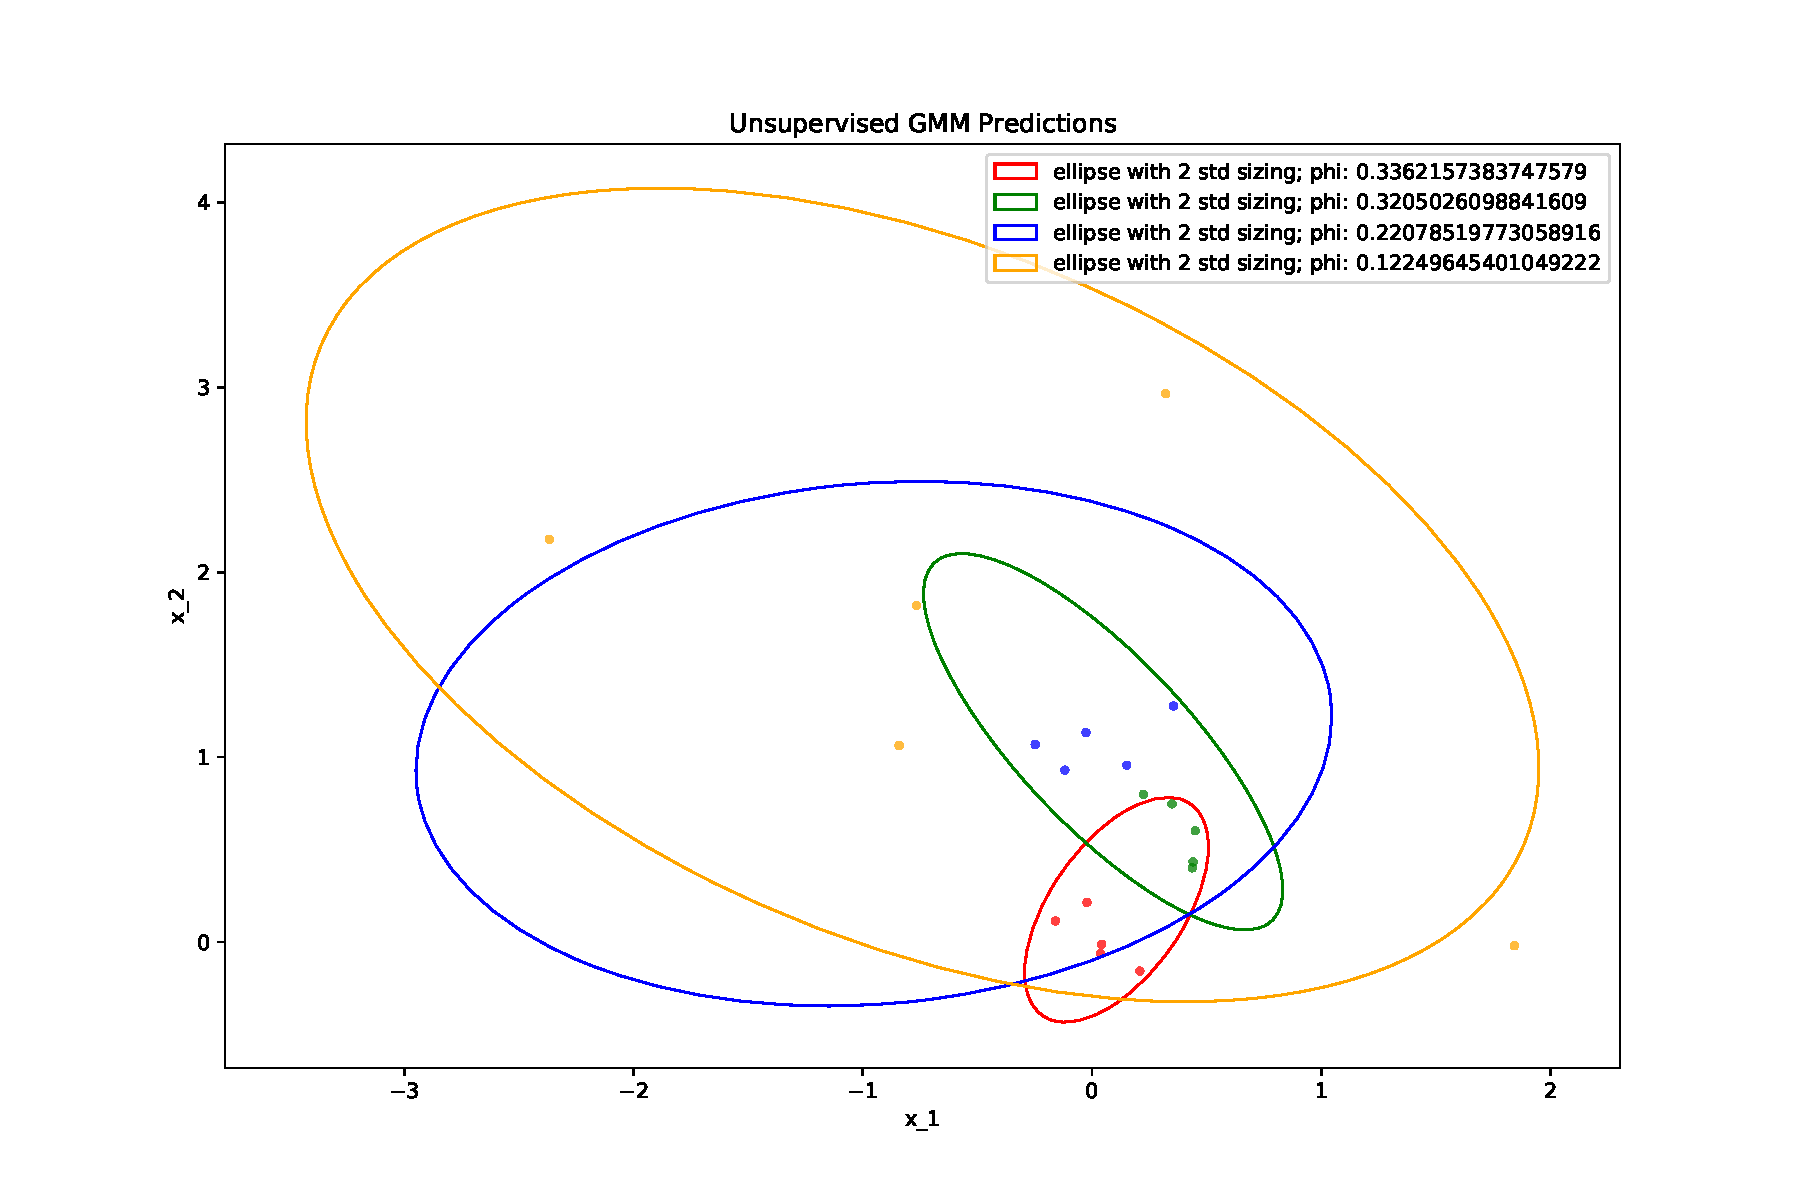
\includegraphics[width=15cm,height=9cm,keepaspectratio]{../src/semi_supervised_em/pred_labelled.pdf}
\end{figure}

Plotting the semi supervised predicted gaussian distributions against the 20 labelled points, and noting the note on the true distribution being 3 low variance gaussians and one high variance. So we see that the semi supervised prediction was better in capturing this than the unsupervised, but still not perfect - it only hits 2 out of the 3 low variance gaussians. We see that it mistakenly has the blue labelled points' ellipse blown up much bigger than the low variance. We somehow ended up with the red ellipse cannabilising some of the unlabelled green points, the green ellipse totally cannabilising the unlabelled blue points, and the blue ellipse left to blow up massively, still covering okishly its' labelled blue points.

The problem above is the small number of supervised points, only 20 compared to 980 unsupervised. At least we have a good spread between clusters.
We can try to fix this by adjusting the weight $\alpha$, increasing it to try to force the blue gaussian smaller to truly capture its cluster. This works - plotted are for $\alpha=40$ and $\alpha=80$ - we see the blue gaussian shrinking and then subsequently pretty well fitting its true cluster

\begin{figure}[H]
	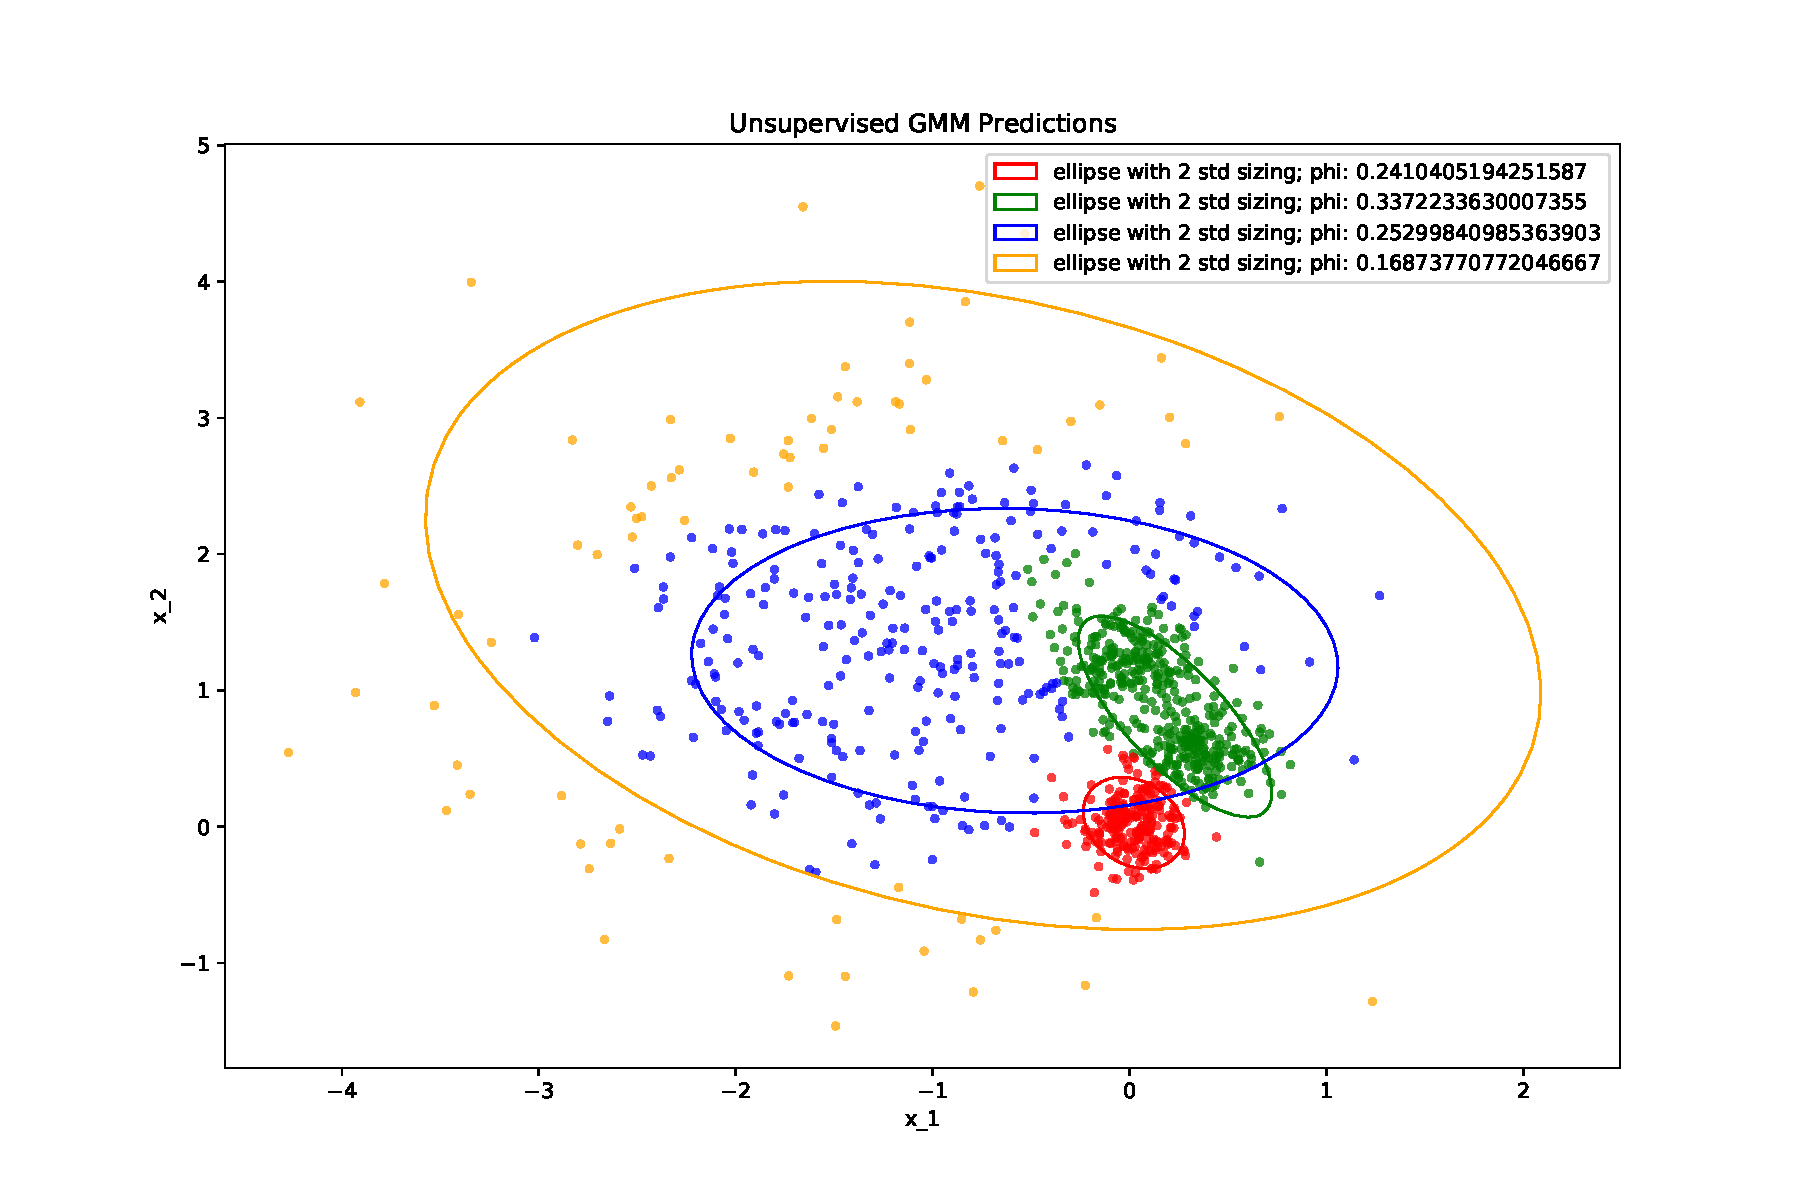
\includegraphics[width=15cm,height=9cm,keepaspectratio]{../src/semi_supervised_em/pred_alpha_40_ss.pdf}
\end{figure}

\begin{figure}[H]
	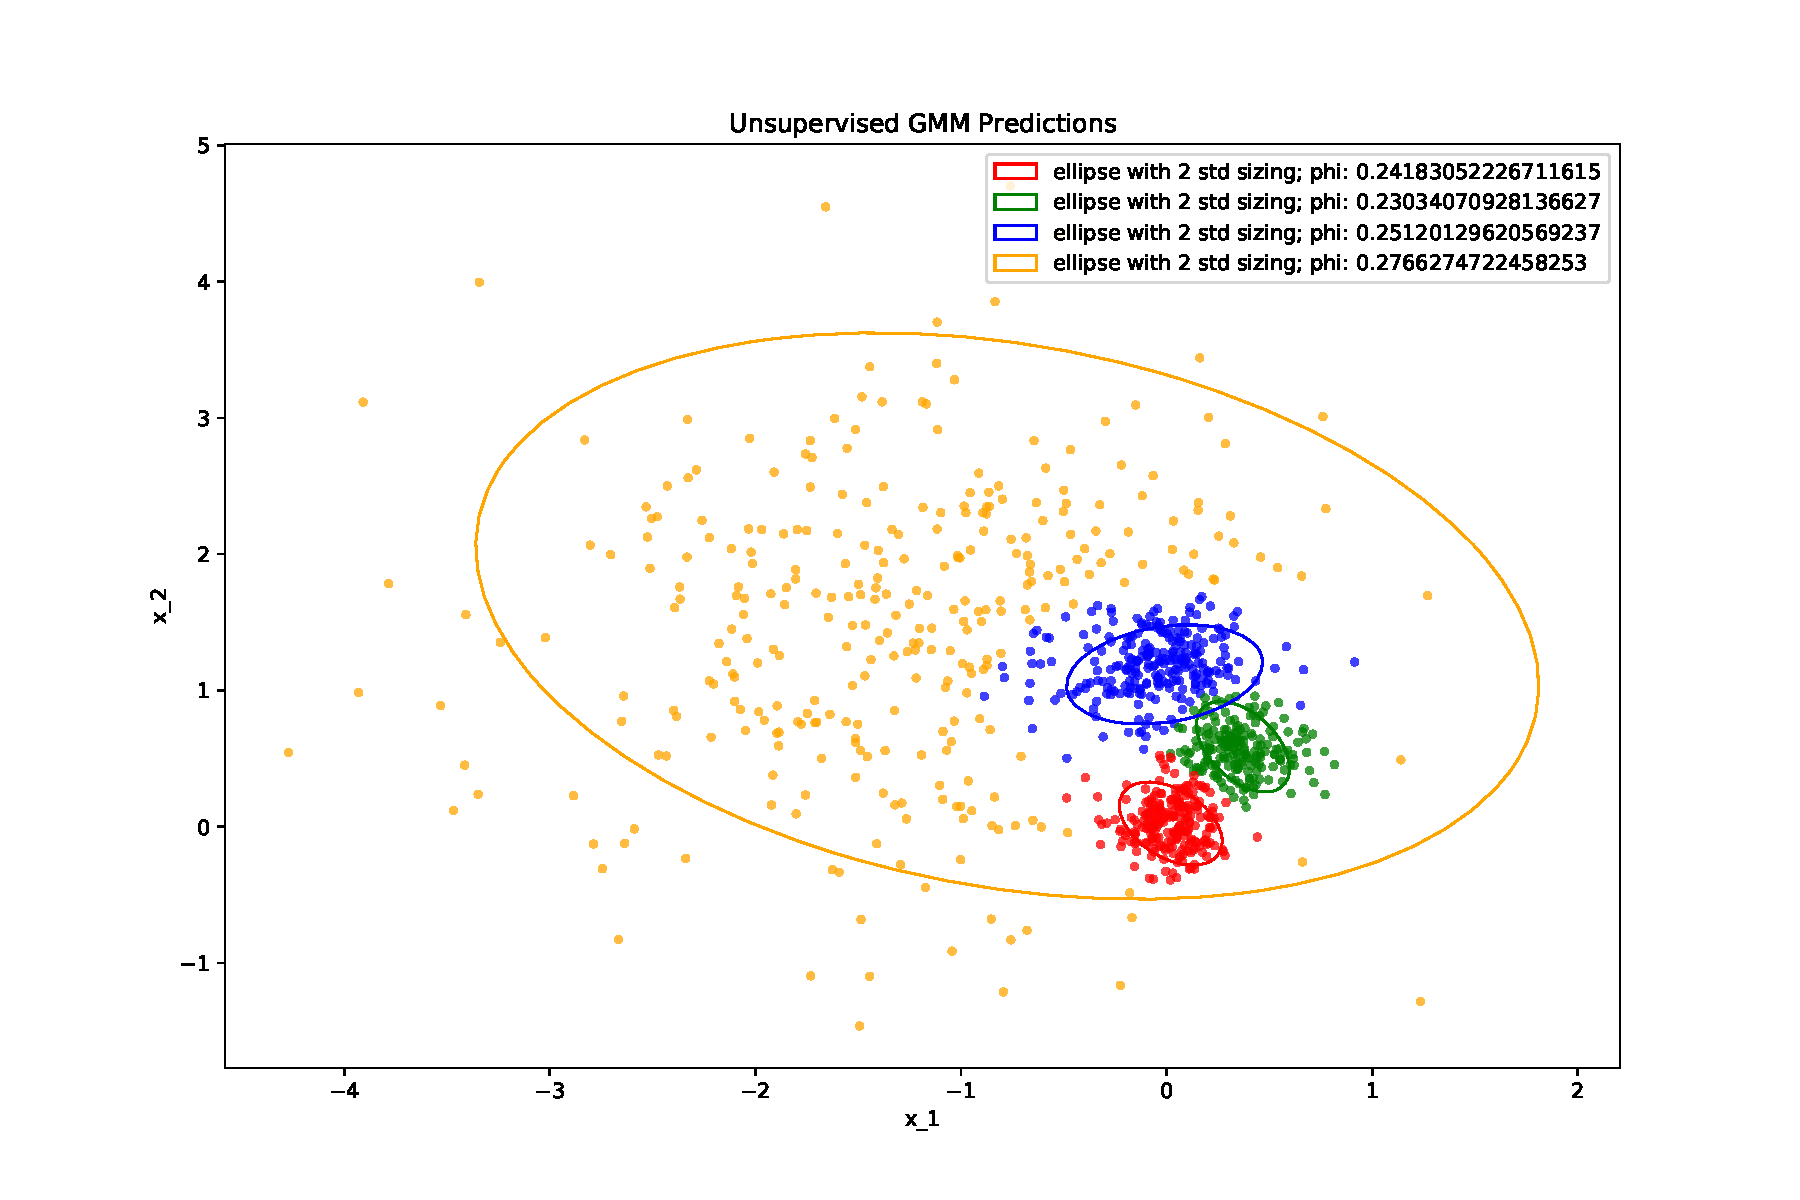
\includegraphics[width=15cm,height=9cm,keepaspectratio]{../src/semi_supervised_em/pred_alpha_80_ss.pdf}
\end{figure}

\end{answer}
